\section{流形的拓扑性质}
\label{sec:mfd-topology}

流形首先是拓扑空间，第~\ref{chap:topological-spaces}章关于连通性与紧性的一般结论都适用。这里只问一个问题：每点附近像欧氏空间这一局部条件，会给整体性质带来什么新结论？下面看两处：连通与路径连通在流形上不再需要区分，紧流形可以用有限张坐标图覆盖。这些结论对带边界流形同样成立，因为半空间中的半球也像欧氏球那样可以用线段连接。

\subsection{连通与路径连通}
\label{sec:mfd-connectedness}

回忆两种概念的区别：连通指空间不能分成两个不相交的非空开集，路径连通指任意两点都能用连续路径连接。路径连通总蕴含连通，反过来一般不成立。

典型反例是拓扑学家的正弦曲线，即曲线$\{(y_1,\sin(1/y_1)):0<y_1\leq1\}$与竖直线段$\{0\}\times[-1,1]$的并，如图~\ref{fig:mfd-connected-sine}(b)所示。曲线越靠近竖直线段振荡越快，竖线上每一点都是曲线上点的极限，所以两部分不能被开集分开，集合连通。但从竖直线段上的点出发，没有连续路径能走到曲线部分。

\begin{BookInlineFigure}
  \centering
  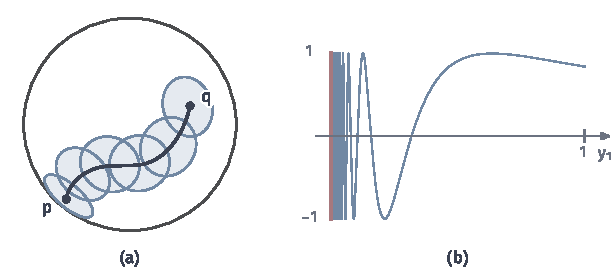
\includegraphics[width=104mm]{figures/04-spaces-measures-and-geometry/04-manifolds/matplotlib/mfd-connected-sine/figure.pdf}
  \caption{局部的线段连接与它失效的情形。(a)球面上连接$p,q$的路径（黑线）由一串相互重叠的坐标球（蓝）接力完成，每个坐标球内部都能用线段走通。(b)拓扑学家的正弦曲线$y_2=\sin(1/y_1)$（蓝）与竖直线段（红）的并。竖线上任意一点的小邻域都含有无穷多段互不相连的弧，所以这里没有路径连通的邻域。}
  \label{fig:mfd-connected-sine}
\end{BookInlineFigure}

\paragraph{局部路径连通}
流形上情况要好得多，因为每点附近都是欧氏的。取包含$p$的坐标图$(U,\varphi)$，在$\varphi(U)$中取以$\varphi(p)$为中心的开球$B$，称$\varphi^{-1}(B)$为\term{坐标球}（coordinate ball）。

球中任意两点$\bm a,\bm b$用线段$t\mapsto(1-t)\bm a+t\bm b$连接，线段留在球内，再用$\varphi^{-1}$送回流形，就得到坐标球内连接两点的连续路径。带边界的情形用半球代替球，半球同样是凸集，线段仍留在其中。于是每点都有任意小的路径连通邻域，这一性质称为\term{局部路径连通}（locally path-connected）。

\begin{theorem}[流形上连通与路径连通等价]
\label{thm:mfd-connected-path-connected}
设$M$是拓扑流形或带边界拓扑流形。则$M$连通当且仅当$M$路径连通。更一般地，$M$的每个路径分支都是既开又闭的集合，并且路径分支与连通分支一致。
\end{theorem}

证明的想法如图~\ref{fig:mfd-connected-sine}(a)：从一点出发能走到的地方，每个点周围都还有一个坐标球能走，所以这个范围不会有“边缘”。

\begin{proof}
设$C$是一个路径分支，即与某点有路径相连的全部点组成的集合。对$q\in C$，取$q$的坐标球$B_q$。$B_q$中每一点都能先连到$q$，再从$q$连到$C$的起点，所以$B_q\subseteq C$，$C$是开集。

不同路径分支互不相交，$C$的补集是其余路径分支的并，也是开集，所以$C$又是闭集。若$M$连通，它唯一的非空既开又闭子集是自身，于是$C=M$，$M$路径连通。反方向是一般拓扑空间中已有的结论。

最后比较两种分支。路径分支$C$路径连通，因而连通，含于某个连通分支$D$。$C$在$D$中既开又闭且非空，$D$连通，所以$C=D$。
\end{proof}

证明只用到“每点有路径连通的邻域”。正弦曲线在竖直线段上的点处缺少这样的邻域，这也说明它不是流形，不能拿来否定定理~\ref{thm:mfd-connected-path-connected}。

\paragraph{连通分支的个数}
每个连通分支是开集，因而本身也是同维流形。第二可数性还限制了分支的个数：每个分支都含有可数基中的某个非空基元素，不同分支所含的基元素不同，所以分支至多可数。

例如双曲线$\{\bm y\in\mathbb R^2:y_2^2-y_1^2=1\}$有上下两个连通分支，每个分支同胚于$\mathbb R$。连通分支数这一整体信息后来由零维同调记录，见第~\ref{chap:homology}章。

\subsection{紧性}
\label{sec:mfd-compactness}

紧空间的任意开覆盖都有有限子覆盖，紧空间上的连续实值函数取得最大值和最小值。这两条在流形上有直接用途。前者让我们只用有限张坐标图处理整个紧流形；后者保证球面上的高度函数$\bm y\mapsto y_3$在某些点达到最高和最低，第~\ref{sec:mfd-smooth-functions}小节将用坐标验证这些点处微分为零。

\paragraph{有限个坐标图}
所有坐标图的定义域组成$M$的一个开覆盖。若$M$紧，就能从中选出有限张图覆盖$M$。圆周用两张图，球面用两张球极投影图，环面用四张乘积图。很多构造先在每张图上局部完成，再把结果拼起来；图的张数有限时，拼接中的求和、取最大值等操作都只涉及有限项。

\paragraph{有限张图不等于一张图}
紧性只给出有限张图，不能推出一张图就够。实际上，正维数的非空紧无边界流形一定不能由单张坐标图覆盖。

证明很短。假设$\varphi:M\to\widehat U$是覆盖整个$M$的坐标图。$\widehat U=\varphi(M)$是紧集的连续像，因而是$\mathbb R^n$中的有界闭集。它又是非空开集，于是是$\mathbb R^n$中非空的既开又闭子集。$\mathbb R^n$连通，所以$\widehat U=\mathbb R^n$，这与有界矛盾。

因此圆周、球面和环面都至少需要两张图。本章开头经纬度在两极失效，问题不在经纬度选得不好，而在于球面的紧性使任何单张坐标图都不可能覆盖全部。

反过来，非紧流形有时一张图就够，例如$\mathbb R^n$。双曲线虽有两个分支，也能用一张图覆盖：在上支令$\varphi(\bm y)=\arctan y_1$，在下支令$\varphi(\bm y)=\arctan y_1+4$，两支分别被送到不相交的开区间$(-\pi/2,\pi/2)$与$(4-\pi/2,4+\pi/2)$。欧氏开集本来就不必连通。单张图能否覆盖整个流形，等于问整个流形能否同胚于一个欧氏开集，紧性只是排除这种可能的一个充分原因。
